% Provenance (never printed): see sources/outline_sources.md (Year 3:
% spectral signatures; optical, thermal and radar sensors; radar
% interferometry; digital elevation models; GIS operations).
% Brief: sources/book5/BRIEFS.md, ch. 25. Curves from figdata/bachelor-3/
% spectral_signatures.py (ECOSTRESS spectra and the Landsat 8 OLI bands),
% thermal_ir.py (Planck's law, brightness temperatures, a mixed pixel),
% insar_mogi.py (the wrapped interferogram of a Mogi source) and
% varden_gis.py (slope, aspect and an overlay on the Varden Hills, from
% figdata/shared/region.py, read only). Exercise and problem values in the
% Book 5 scratch calculator calc/ch25.py. Mount Halvren, its lava flows and
% its fumaroles are invented. The brief's overlay (slope > 15 degrees on
% limestone within 200 m of the river) is empty on the Varden model: the
% valley floor is flat; the printed overlay uses the shale within 1 km.
\chapter{遥感与地理信息系统}\label{ch:b3:remote-sensing-gis}

1997 年，喀斯喀特山脉中一处荒野的地面开始隆起，该处靠近
一组名为“三姐妹”的火山群。到 2001 年，隆起中心已高出
\qty{15}{cm}。隆起正上方并无火山，该地区
最近一次喷发距今已有 1500 年。隆起并非由人在其上行走时发现，
而是在将该地区的雷达图像合并后，显现为一组彩色环纹，形似牛眼；
这些图像取自轨道，拍摄时间相隔数年。
环纹显示，侵入的岩浆位于地下 6 至 \qty{7}{km} 处；2004 年 3 月，
一场由 300 多次小地震组成的震群发生于其中心附近。
本章说明卫星如何在数百千米高空，测出仅几
厘米的变化；轨道上的其他传感器能看到
地表的哪些情况，以及这些传感器所制地图如何
在地理信息系统中组合。
% ledger: usgs:insar-fs

\begin{recall}
电磁波谱、黑体的普朗克定律、发射率
以及基尔霍夫定律、反射率与波的干涉，见于物理教材；
遥感、卫星图像、地图投影与卫星定位，
见于中学教材。大气窗口与测光波段，
见于本科一年级分册的望远镜一章；数字高程模型，
以及存储它的地理信息系统，
见于其地质图一章；第一幅地震位移的雷达图，
见于其地震源一章。膨胀岩浆储库的
茂木源，见于本科二年级分册的
火山喷发一章。
\end{recall}

\section{光谱特征与光学传感器}\label{sec:b3:remote-sensing-gis:optical}

到达地面的太阳光一部分被吸收，一部分被反射，
其比例取决于波长，以及地面
由何种物质构成。轨道上的传感器在若干波长范围内测量反射光，
这些范围称为波段，波段之间的比值可用于识别
地表。

\begin{definition}[光谱特征]\label{def:b3:remote-sensing-gis:signature}
称物质的\emph{光谱特征}\index{光谱特征}为
其反射率随波长的函数 $R(\lambda)$，即
它所反射的入射辐射的比例。在热红外波段，
表面主要发射而非反射，此时光谱特征为发射率
$\varepsilon(\lambda)$；对于不透明样品，$\varepsilon = 1 - R$。
\end{definition}

\begin{omfigure}
\centering
\begin{tikzpicture}
\begin{axis}[width=0.9\linewidth, height=6.4cm, xmin=0.4, xmax=2.5, ymin=0, ymax=1,
  xlabel={波长 (\unit{\micro\metre})}, ylabel={反射率},
  tick label style={font=\scriptsize}, label style={font=\small},
  legend style={font=\scriptsize, at={(0.5,-0.24)}, anchor=north, /tikz/every even column/.append style={column sep=4pt}},
  legend columns=5, clip=false]
\fill[black!8] (axis cs:0.45,0) rectangle (axis cs:0.51,1);
\fill[black!8] (axis cs:0.53,0) rectangle (axis cs:0.59,1);
\fill[black!8] (axis cs:0.64,0) rectangle (axis cs:0.67,1);
\fill[black!8] (axis cs:0.85,0) rectangle (axis cs:0.88,1);
\fill[black!8] (axis cs:1.57,0) rectangle (axis cs:1.65,1);
\fill[black!8] (axis cs:2.11,0) rectangle (axis cs:2.29,1);
\addplot[very thick, green!50!black] table[x=um, y=grass] {figdata/out/bachelor-3-spectral_signatures-spectra.dat};
\addlegendentry{绿草}
\addplot[thick, brown!70!black, dashed] table[x=um, y=soil] {figdata/out/bachelor-3-spectral_signatures-spectra.dat};
\addlegendentry{棕色沙质土壤}
\addplot[thick, black!55] table[x=um, y=kaol] {figdata/out/bachelor-3-spectral_signatures-spectra.dat};
\addlegendentry{高岭石}
\addplot[thick, red!70!black, dash dot] table[x=um, y=hem] {figdata/out/bachelor-3-spectral_signatures-spectra.dat};
\addlegendentry{赤铁矿}
\addplot[thick, omDef] table[x=um, y=water] {figdata/out/bachelor-3-spectral_signatures-spectra.dat};
\addlegendentry{水}
\node[font=\tiny, anchor=south] at (axis cs:0.48,1) {2};
\node[font=\tiny, anchor=south] at (axis cs:0.56,1) {3};
\node[font=\tiny, anchor=south] at (axis cs:0.655,1) {4};
\node[font=\tiny, anchor=south] at (axis cs:0.865,1) {5};
\node[font=\tiny, anchor=south] at (axis cs:1.61,1) {6};
\node[font=\tiny, anchor=south] at (axis cs:2.2,1) {7};
\end{axis}
\end{tikzpicture}
\par\smallskip{\small 五种地表的实验室反射光谱（ECOSTRESS
Spectral Library，经 Jet Propulsion
Laboratory, California Institute of Technology 许可转载），图中以阴影标出六个
反射波段，即 Landsat~8 与 9 成像仪的第 2 至 7 波段。绿草在
可见光中暗，在近红外中最亮；高岭石处处明亮，
仅在 \qty{2.2}{\micro\metre} 处有一狭窄吸收；赤铁矿吸收蓝光与绿光，
并反射红光；水在各波长处仅反射
百分之几。}\label{fig:b3:remote-sensing-gis:spectra}
\end{omfigure}
% ledger: data:b5-ecostress, usgs:landsat8-bands, nasa:ndvi

上图中的\omterm{def:b3:remote-sensing-gis:signature}{光谱特征}，是光学遥感的
词汇。叶片中的叶绿素在 0.4 与
\qty{0.7}{\micro\metre} 之间强烈吸收，用于光合作用；而叶片细胞
在 0.7 至 \qty{1.1}{\micro\metre} 之间强烈反射：绿草
在 第 4 波段 的红光中反射 \qty{5}{\percent}，在 第 5 波段 的
近红外中反射 \qty{50}{\percent}，这一跃升为岩石与土壤所不具备。在更远处，两个
低谷位于 1.4 与 \qty{1.9}{\micro\metre} 附近，是液态水的吸收处。
棕色沙质土壤的反射率向红外方向稳步升高。高岭石，
一种黏土，在可见光中呈白色，并在
\qty{2.20}{\micro\metre} 处有一狭窄吸收，位于 第 7 波段 内，使其在该波段比
第 6 波段 更暗；\omterm{def:b3:remote-sensing-gis:sensors}{高光谱传感器}可分辨其形状，并将一种黏土与
另一种区分开来。赤铁矿吸收蓝光与绿光，因此呈红色。
% ledger: nasa:ndvi, data:b5-ecostress

\begin{definition}[空间分辨率、光谱分辨率、辐射分辨率与重访周期]\label{def:b3:remote-sensing-gis:resolutions}
图像的\emph{空间分辨率}\index{空间分辨率}是其
一个像元在地面上的尺寸。其\emph{光谱
分辨率}\index{光谱分辨率}是其波段的数目与宽度，其
\emph{辐射分辨率}\index{辐射分辨率}是每次测量所记录的
等级数，即 $2^b$，$b$ 为比特数。
卫星的\emph{重访周期}\index{重访周期}是
它两次对同一地点观察之间的时间间隔。
\end{definition}

四者不可能同时都很精细：更小的像元与更窄的波段
各自收集的光更少，而更窄的幅宽需要更长时间才能覆盖
整个地球。Landsat~8 成像仪于 2013 年发射，共九个波段，其中大部分
的像元为 \qty{30}{m}，另有一个全色波段，像元为 \qty{15}{m}；它
记录 4096 个等级（12 比特），而 Landsat 1 至 7 的仪器
只记录 256 个。它在 \qty{705}{km} 高的太阳同步轨道上成像，
幅宽 \qty{185}{km}，每 16 天重访同一地面；
Landsat~9 与之位于同一轨道，两者相隔 8 天，使重访等待时间减半。
每颗 Sentinel-2 卫星的多光谱成像仪有 13 个波段，像元分别为 10、20
或 \qty{60}{m}，幅宽 \qty{290}{km}；若两颗卫星位于同一轨道，
则赤道处的\omterm{def:b3:remote-sensing-gis:resolutions}{重访周期}为 5 天。
% ledger: usgs:landsat8-bands, usgs:landsat8-orbit, esa:s2-msi, esa:s2-orbit

\begin{definition}[多光谱与高光谱传感器]\label{def:b3:remote-sensing-gis:sensors}
\emph{多光谱传感器}\index{多光谱传感器}记录数个
至数十个彼此间隔的波段。\emph{高光谱
传感器}\index{高光谱传感器}记录许多窄且相邻的波段，
使每个像元都带有近似连续的光谱，可与
上图那样的光谱库相比较。
\end{definition}

地面与传感器之间是大气。它会把从未触及地面的
太阳光散射进传感器，且以短波长为甚，
这部分称为程辐射；它还会吸收地面反射光的
一部分，尤其是在大气窗口之外的波段。

\begin{definition}[大气校正]\label{def:b3:remote-sensing-gis:atm-correction}
\emph{大气校正}\index{大气校正}是
将在大气层顶测得的辐亮度转换为
地表反射率，方法是扣除程辐射，并
抵消光线往返两段路径（向下与向上）上的吸收。
\end{definition}

最简单的校正是在每个波段中减去场景中最暗像元的值，
这些像元可为深而澄清的水体或阴影，它们本应几乎不反射任何光：
其所示的正是程辐射。精细的校正还会对
大气中的分子、气溶胶和水蒸气进行建模。

\begin{definition}[归一化植被指数]\label{def:b3:remote-sensing-gis:ndvi}
某像元的\emph{归一化植被
指数}\index{归一化植被指数}（NDVI）为
\[
\mathrm{NDVI} = \frac{R_\mathrm{NIR} - R_\mathrm{red}}{R_\mathrm{NIR} + R_\mathrm{red}} ,
\]
由其在一个近红外波段与一个红光波段中的反射率计算得到。
\end{definition}

该指数介于 $-1$ 与 $+1$ 之间。无绿叶的地面给出
接近零的值：裸岩、沙或雪为 \num{0.1} 及以下，
灌木与草地为 0.2 至 0.3，温带与热带雨林为 0.6 至
0.8；最茂密的绿叶接近 0.8 至 0.9。由上图的光谱，
经波段 4 与 5 计算，草地为 0.82，棕色沙土为
0.15，水体为 $-0.01$。作为比值，该指数在
两个波段以相同比例变暗时不会改变，例如背光坡面所致的
或均匀薄霾所致的变暗：它度量的是植被，而非
光照。加性的程辐射在红光中更大，会改变它，
这正是该指数须由校正后反射率计算的原因
（见\cref{exo:b3:remote-sensing-gis:12}）。
% ledger: nasa:ndvi, data:b5-ecostress

\section{热红外}\label{sec:b3:remote-sensing-gis:thermal}

地面温度约为 \qty{300}{K} 时，普朗克定律给出
黑体发射的峰值位于 \qty{9.7}{\micro\metre} 附近，位于
热红外的大气窗口之中。在此处，传感器测得的是
地表发出的辐射，而非其反射的辐射。Landsat~8 的热红外传感器
有两个波段，分别为 10.6 至 11.19 与 11.5 至 \qty{12.51}{\micro\metre}，
像元为 \qty{100}{m}。
% ledger: const:h, const:c, const:kB, usgs:landsat8-bands

\begin{definition}[亮度温度]\label{def:b3:remote-sensing-gis:brightness}
某表面的\emph{亮度温度}\index{亮度温度} $T_b$，
在波长 $\lambda$ 处，是指能发出
该波长处实测光谱辐亮度 $L$ 的黑体温度。
而\emph{动力学温度}是该表面的
热力学温度，即温度计所读出的温度。
\end{definition}

\begin{proposition}[由辐亮度求亮度温度]\label{prop:b3:remote-sensing-gis:planck-inversion}
设 $c_1 = 2hc^2$，$c_2 = hc/k$，光谱辐亮度 $L$ 在
波长 $\lambda$ 处的\omterm{def:b3:remote-sensing-gis:brightness}{亮度温度}为
\[
T_b = \frac{c_2}{\lambda \ln\!\left(1 + \dfrac{c_1}{\lambda^5 L}\right)} .
\]
发射率为 $\varepsilon < 1$、动力学温度为 $T$ 的表面，
其发出的辐亮度为 $L = \varepsilon B_\lambda(T)$，且其\omterm{def:b3:remote-sensing-gis:brightness}{亮度温度} $T_b < T$。
\end{proposition}

\begin{proof}
由普朗克定律得 $B_\lambda(T) = c_1\lambda^{-5}/(e^{c_2/\lambda T} -
1)$。令 $B_\lambda(T_b) = L$，解得 $e^{c_2/\lambda T_b} = 1 +
c_1/(\lambda^5L)$，即为上式。$B_\lambda$ 随
温度升高而增大，故由 $\varepsilon B_\lambda(T) < B_\lambda(T)$ 可得 $T_b < T$。
\end{proof}
% ledger: const:h, const:c, const:kB

这一差异很重要。在 第 10 波段 中心，即 \qty{10.9}{\micro\metre} 处，
若表面温度为 \qty{300}{K}、发射率为 0.95，则其\omterm{def:b3:remote-sensing-gis:brightness}{亮度温度}
为 \qty{296.6}{K}；发射率为 0.99 时为 \qty{299.3}{K}，发射率
相差百分之一，便足以造成超过半开尔文的差异。实验室光谱给出，
在 第 10 波段 中，草地的发射率为 0.98，水体为 0.99，
棕色沙土为 0.97。因此，从轨道绘制温度图需要
每个像元的发射率，并需对两者之间空气的发射与
吸收进行校正。
% ledger: data:b5-ecostress

\begin{omfigure}
\centering
\begin{tikzpicture}
\begin{groupplot}[group style={group size=2 by 1, horizontal sep=1.5cm},
  width=0.48\linewidth, height=0.42\linewidth,
  tick label style={font=\scriptsize}, label style={font=\small}, title style={font=\small}]
\nextgroupplot[title={黑体辐射亮度}, xmode=log, ymode=log, xmin=1, xmax=25,
  ymin=0.01, ymax=1e5, xlabel={波长 (\unit{\micro\metre})},
  ylabel={$B_\lambda$ (\unit{W.m^{-2}.sr^{-1}.\micro\metre^{-1}})},
  xtick={1,2,5,10,20}, xticklabels={1,2,5,10,20}]
\fill[black!10] (axis cs:10.6,0.01) rectangle (axis cs:11.19,1e5);
\fill[black!10] (axis cs:2.11,0.01) rectangle (axis cs:2.29,1e5);
\addplot[thick, omDef] table[x=um, y=b300] {figdata/out/bachelor-3-thermal_ir-planck.dat};
\addplot[thick, omDef, dashed] table[x=um, y=b400] {figdata/out/bachelor-3-thermal_ir-planck.dat};
\addplot[thick, red!70!black] table[x=um, y=b1443] {figdata/out/bachelor-3-thermal_ir-planck.dat};
\node[font=\scriptsize, omDef, anchor=north east] at (axis cs:24,3) {\qty{300}{K}};
\node[font=\scriptsize, omDef, anchor=south west] at (axis cs:12.5,30) {\qty{400}{K}};
\node[font=\scriptsize, red!70!black, anchor=south west] at (axis cs:3.2,2000) {\qty{1443}{K}};
\node[font=\tiny, anchor=north] at (axis cs:10.9,1e5) {10};
\node[font=\tiny, anchor=north] at (axis cs:2.2,1e5) {7};
\nextgroupplot[title={混合像元，波段 10}, xmin=0, xmax=1, ymin=285, ymax=375,
  xlabel={像元中温度为 \qty{370}{K} 的部分所占比例 $f$}, ylabel={温度 (\unit{K})},
  legend style={font=\scriptsize, at={(0.97,0.03)}, anchor=south east}]
\addplot[thick, red!70!black] table[x=f, y=tb] {figdata/out/bachelor-3-thermal_ir-mixed.dat};
\addlegendentry{亮度温度}
\addplot[thick, black!60, dashed, domain=0:1] {290 + 80*x};
\addlegendentry{平均温度}
\end{groupplot}
\end{tikzpicture}
\par\smallskip{\small 左图为 300 和 \qty{400}{K} 表面的普朗克定律，
以及 \qty{1170}{\celsius}（即 \qty{1443}{K}）火山喷发熔岩的普朗克定律，
并以阴影标出 Landsat~8 的短波红外波段~7 和热红外波段~10。
右图为像元在波段~10 中的\omterm{def:b3:remote-sensing-gis:brightness}{亮度温度}，该像元中比例为
$f$ 的部分温度为 \qty{370}{K}，其余为 \qty{290}{K}，并与
按面积加权的平均温度相比：热部分的权重超过了它的
面积占比。}\label{fig:b3:remote-sensing-gis:thermal}
\end{omfigure}
% ledger: const:h, const:c, const:kB, usgs:landsat8-bands, usgs:kilauea-temp

温度为 \qty{1170}{\celsius} 的熔岩，其峰值位于 \qty{2.0}{\micro\metre} 附近：一股
远小于一个像元的新鲜熔岩流，会点亮光学成像仪的短波红外
波段，无论白天或夜间。像元很少是均匀的，而且
普朗克定律关于温度并非线性。
% ledger: usgs:kilauea-temp

\begin{proposition}[混合像元]\label{prop:b3:remote-sensing-gis:mixed}
像元中比例为 $f$ 的部分以温度 $T_h$ 的黑体形式发射，其余部分
温度为 $T_0 < T_h$，其辐射亮度为 $L = fB_\lambda(T_h) + (1 - f)B_\lambda(T_0)$，
且当 $0 < f < 1$ 时，其\omterm{def:b3:remote-sensing-gis:brightness}{亮度温度}超过按面积加权的
平均温度 $fT_h + (1 - f)T_0$。
\end{proposition}

\begin{proof}
辐射亮度是各部分辐射亮度按面积的加权平均。记 $B_\lambda(T)
= c_1\lambda^{-5}g(c_2/\lambda T)$，其中 $g(x) = 1/(e^x - 1)$；
以 $T$ 为变量，记 $x = c_2/\lambda T$，则
$g(c_2/\lambda T)$ 的二阶导数为 $(x g''(x) + 2g'(x))\,x/T^2$，当 $x(e^x + 1)
> 2(e^x - 1)$ 时为正，即 $x > 2\tanh(x/2)$，对每个 $x > 0$ 均成立：
$B_\lambda$ 关于 $T$ 为凸。由凸性可知
各辐射亮度的平均值大于平均温度对应的辐射亮度，
又 $B_\lambda$ 随 $T$ 增大，故 $T_b > fT_h + (1 - f)T_0$。
\end{proof}

像元中有 \qty{5}{\percent} 的部分
为温度 \qty{370}{K} 的喷气孔地面，其余为 \qty{290}{K} 的背景，
则其平均温度为 \qty{294}{K}，而\omterm{def:b3:remote-sensing-gis:brightness}{亮度温度}为 \qty{295.3}{K}；
比例为 \qty{10}{\percent} 时为 \qty{300.4}{K}。热点在热红外
图像中十分突出，其温度不能仅由一个波段读出：两个
不同波长的波段给出关于 $f$ 和 $T_h$ 的两个方程。

\section{雷达与激光雷达}\label{sec:b3:remote-sensing-gis:radar}

光学或热红外传感器是被动式的：它测量地面
发出的光。雷达与\omterm{def:b3:remote-sensing-gis:lidar}{激光雷达}是主动式的：它发出脉冲，并测量其回波的时间。
微波可以穿过云层，雷达自带照明，
因此它在任何天气下都能昼夜观测。
% ledger: esa:s1-sar

\begin{definition}[合成孔径雷达；雷达后向散射]\label{def:b3:remote-sensing-gis:sar}
称\emph{合成孔径雷达}\index{合成孔径雷达}（SAR）为
沿航迹搭载、向侧方观测的雷达，它将沿航迹一段长度内
从地面同一点记录到的回波加以组合，并保留其相位，
仿佛这些回波是由一根与该段等长的天线接收的一样。
地表的\emph{雷达后向散射}\index{雷达后向散射}，是其接收功率中
向天线方向散射回去的部分所占的
比例。
\end{definition}

\begin{omfigure}
\centering
\begin{tikzpicture}[>=stealth, font=\small, x=1cm, y=1cm]
\fill[black!12] (-0.5,-0.35) rectangle (10.5,0);
\draw[thick] (-0.5,0) -- (10.5,0);
% satellite
\fill[omDef] (0.6,4.6) rectangle (1.4,5.0);
\draw[thick, omDef] (0.35,4.45) -- (1.65,5.15);
\draw (1.0,4.8) circle (0.12); \fill (1.0,4.8) circle (0.03);
\node[font=\scriptsize, anchor=south, align=center] at (1.0,5.3) {飞行方向（方位角）\\指入纸面};
% nadir
\draw[dashed, black!60] (1.0,4.4) -- (1.0,0);
\node[font=\scriptsize, anchor=north] at (1.0,-0.4) {天底};
\draw[<->, black!60] (0.3,0) -- node[left, font=\scriptsize] {$h$} (0.3,4.4);
% beam
\fill[omDef!12] (1.0,4.4) -- (4.3,0) -- (9.6,0) -- cycle;
\draw[omDef!60] (1.0,4.4) -- (4.3,0); \draw[omDef!60] (1.0,4.4) -- (9.6,0);
\node[font=\scriptsize, anchor=north] at (4.3,-0.4) {近距};
\node[font=\scriptsize, anchor=north] at (9.6,-0.4) {远距};
\draw[<->] (4.3,-1.0) -- node[below, font=\scriptsize] {测绘带} (9.6,-1.0);
% target and slant range
\fill[red!70!black] (7.0,0) circle (0.07);
\draw[thick, red!70!black] (1.0,4.4) -- node[above, sloped, font=\scriptsize] {斜距 $R$} (7.0,0);
\draw[black!60] (7.0,0) -- (7.0,1.8);
\draw[black!60] (7.0,0.9) arc (90:126.25:0.9);
\node[font=\scriptsize] at (6.6,1.2) {$\theta$};
\draw[->, very thick, omThm] (7.0,0) -- (6.2,0.59) node[anchor=north east, font=\scriptsize, inner sep=1pt] {LOS};
\draw[<->, black!60] (1.0,-1.6) -- node[below, font=\scriptsize] {地距} (7.0,-1.6);
\draw[black!60] (1.0,-1.5) -- (1.0,-1.7); \draw[black!60] (7.0,-1.5) -- (7.0,-1.7);
\end{tikzpicture}
\par\smallskip{\small 侧视雷达的几何关系，示于
与航迹垂直的平面内。波束照亮天底一侧的
测绘带；地面某点以斜距 $R$ 被观测到，入射角为
$\theta$，沿\omterm{def:b3:remote-sensing-gis:insar}{视线方向}（LOS）。回波按
其横越航迹的延迟（距离向）分类，并按
沿航迹合成孔径的相位历史（方位向）分类。}\label{fig:b3:remote-sensing-gis:sar}
\end{omfigure}

\begin{proposition}[方位向分辨率]\label{prop:b3:remote-sensing-gis:azimuth}
长度为 $L$ 的真实天线在斜距 $R$ 处，
沿航迹方向只有相距大于约 $R\lambda/L$ 的两点才能被分辨；
同一天线的\omterm{def:b3:remote-sensing-gis:sar}{合成孔径雷达}可达约 $L/2$，
与距离无关。
\end{proposition}

\begin{proof}
长度为 $L$ 的天线，其波束张开的角度约为
$\lambda/L$，因此沿航迹照亮一条长 $R\lambda/L$ 的带状区域，并且
真实天线无法分辨其中的两点。地面某点在波束中停留，
天线行进同样长度 $\ell = R\lambda/L$ 的过程中，
这就是合成孔径。对 $\ell$ 上的回波进行合并，
等效于长度为 $\ell$ 的天线；每条回波路径都
往返走过一次，使合成天线的波束缩小为
$\lambda/(2\ell)$，分辨率为 $R\lambda/(2\ell) =
L/2$。较远的点在波束中停留更久，更长的合成孔径
恰好抵消了更大的距离。
\end{proof}

每颗 Sentinel-1 卫星的雷达工作在 C 波段，
\qty{5.405}{GHz}，波长约为 \qty{5.55}{cm}，天线
长 \qty{12.3}{m}，位于 \qty{693}{km} 高空。尺寸如此的真实天线
沿航迹方向只能分辨约 \qty{4}{km} 的细节；合成孔径
将 $L/2$ 降至约 \qty{6}{m}。在陆地上，它主要以
宽测绘带模式工作，由三个子带拼接覆盖 \qty{250}{km}，
入射角介于 29 与 \ang{46} 之间，分辨单元为 5 × \qty{20}{m}。
每颗卫星的轨道每 12 天重复一次。
% ledger: esa:s1-sar, esa:s1-orbit, esa:s1-iw

\omterm{def:b3:remote-sensing-gis:sar}{雷达后向散射}取决于地表在波长尺度上的粗糙程度，
以及地表的湿度。平静的湖面将脉冲向外反射，如同
镜子，因而呈黑色；粗糙的熔岩流、森林冠层或由墙体和
拐角组成的城市则将其中大部分送回，呈亮色。

\begin{definition}[激光雷达]\label{def:b3:remote-sensing-gis:lidar}
\emph{激光雷达}\index{激光雷达}通过测量
由地面、植被或水体反射的激光脉冲的飞行时间来测量距离。
\end{definition}

\begin{proposition}[飞行时间]\label{prop:b3:remote-sensing-gis:tof}
脉冲离开后经时间 $t$ 返回，表明它在距离
$ct/2$ 处遇到了地表；时间上的不确定度 $\delta t$ 对应
距离上的不确定度 $c\,\delta t/2$。
\end{proposition}

\begin{proof}
光以速度 $c$ 往返传播，路程为 $2d = ct$。
\end{proof}

ICESat-2 的激光测高仪位于约 \qty{500}{km} 高空，
每秒发射 \num{10000} 个脉冲，波长 \qty{532}{nm}，分为六束，
沿地面每隔 \qty{0.7}{m} 一束，光斑直径 \qty{11}{m}。
每个脉冲射出的约 300 万亿个光子中，只有约十二个
返回，每个光子的计时精度为 \qty{800}{ps}，对应 \qty{12}{cm} 的距离。
在森林上空，一些光子从树冠返回，另一些
则穿过林隙从地面返回：两者之差即树木的高度，而
仅由地面光子即可绘出其下方的地形起伏。机载\omterm{def:b3:remote-sensing-gis:lidar}{激光雷达}
也以同样方式测绘植被覆盖之下的地面。
% ledger: nasa:icesat2-atlas, nasa:icesat2-photons

\section{雷达干涉测量}\label{sec:b3:remote-sensing-gis:insar}

雷达记录的回波具有振幅，即回波的强度，
以及相位，它以
波长为单位计量往返距离。单幅图像的相位本身没有用处：每个像元包含许多
散射体，其回波以随机相位相加。但若地面在此期间没有变化，
同一批散射体便再次给出相同的和。
% ledger: usgs:insar-vhp

\begin{definition}[雷达干涉测量；干涉图；视线方向]\label{def:b3:remote-sensing-gis:insar}
\emph{雷达干涉测量}\index{雷达干涉测量}（InSAR）将
同一地面的两幅雷达图像，两次获取时位置几乎相同，
逐像元进行组合。它们的\emph{干涉图}\index{干涉图}
是两者相位差的图，该相位差以 $2\pi$ 为模已知，并
绘成颜色循环的形式，每个循环即一个\emph{干涉条纹}。\emph{视线
方向}\index{视线方向（雷达）}是从地面指向天线的方向，雷达
只测量位移在此方向上的分量。
\emph{相位解缠}\index{相位解缠}是由卷绕相位
重建连续相位的过程，即给每个像元加上
使相位与邻域平滑变化的 $2\pi$ 整数倍。
\end{definition}

\begin{theorem}[一个干涉条纹]\label{thm:b3:remote-sensing-gis:fringe}
同一位置的两次获取之间，地面的位移使
地面到天线的距离缩短 $\Delta r$，则其回波的
相位改变 $\Delta\phi = 4\pi\Delta r/\lambda$。一个干涉条纹，即相位变化 $2\pi$，
对应沿\omterm{def:b3:remote-sensing-gis:insar}{视线方向} $\lambda/2$ 的位移。
\end{theorem}

\begin{proof}
回波往返经过的路程为 $2r$，其相位为
$2\pi\cdot 2r/\lambda$ 加上由散射体决定的常数，该常数在
两幅图像中相同。相位差为 $4\pi\Delta r/\lambda$，当其等于 $2\pi$ 时，
$\Delta r = \lambda/2$。
\end{proof}

对于 Sentinel-1，一个干涉条纹为 \qty{27.7}{mm}；对于较早的欧洲与
加拿大卫星（波长 \qty{5.66}{cm}），一个干涉条纹为 \qty{28.3}{mm}，
即下图照片中的颜色循环。实际上，两次过境的
位置相差可达一百米左右（Sentinel-1 将其
保持在参考轨道 \qty{120}{m} 之内），而相位差
还包含地形起伏，可由数字高程模型去除；
大气中的水汽在两个日期对电磁波的延迟不同；
而地面在两次过境之间发生变化之处，尤其是植被，
相位失去相干性，条纹便消散为噪声。较长的
L 波段波长 \qty{23.53}{cm}，穿透植被的能力
优于 C 波段。
% ledger: esa:s1-sar, esa:s1-orbit, usgs:insar-fs, photo:b3-three-sisters-insar

\begin{proposition}[沿视线方向所见的茂木源]\label{prop:b3:remote-sensing-gis:mogi-los}
在体积变化为 $\Delta V$、深度为 $z_0$ 的茂木源上方，
水平距离 $r$ 处，地面向上移动 $u_z$（与本科二年级分册相同），并
向外移动，其位移为
\[
u_r = \frac{(1 - \nu)\,\Delta V}{\pi}\,\frac{r}{(r^2 + z_0^2)^{3/2}} = \frac{r}{z_0}\,u_z .
\]
从东侧卫星以入射角 $\theta$ 观测时，\omterm{def:b3:remote-sensing-gis:insar}{视线方向}的变化为
$d = u_E\sin\theta + u_z\cos\theta$，其中 $u_E$ 为
向东位移。沿过中心的南北向直线，
$d = u_z\cos\theta$.
\end{proposition}

\begin{proof}
径向公式与同一解中的竖直公式配套，
从地面指向卫星的单位矢量为
$(\sin\theta, 0, \cos\theta)$，分量依次为东、北、上，视距变化为
位移在其上投影的负值，因此
缩短量即 $d$。在南北向直线上，向外的运动
指向北或南，与该矢量垂直，且 $u_E = 0$。
\end{proof}
% ledger: dmodels:mogi, dmodels:mogi-radial

\begin{omfigure}
\centering
\begin{tikzpicture}
\begin{groupplot}[group style={group size=2 by 1, horizontal sep=1.5cm},
  tick label style={font=\scriptsize}, label style={font=\small}, title style={font=\small}]
\nextgroupplot[title={缠绕干涉图}, width=0.46\linewidth, height=0.46\linewidth,
  axis equal image, enlargelimits=false, xmin=-15, xmax=15, ymin=-15, ymax=15,
  xlabel={东 (km)}, ylabel={北 (km)},
  colormap={fringe}{rgb255=(128,0,170) rgb255=(30,60,220) rgb255=(0,170,220) rgb255=(30,170,60) rgb255=(240,220,0) rgb255=(240,120,0) rgb255=(220,20,30) rgb255=(128,0,170)},
  point meta min=0, point meta max=6.2832]
\addplot[matrix plot*, mesh/cols=101, point meta=explicit] table[x=x, y=y, meta=phase] {figdata/out/bachelor-3-insar_mogi-map.dat};
\draw[->, very thick, white] (axis cs:6,-12.5) -- (axis cs:12,-12.5);
\node[font=\scriptsize, white, anchor=south] at (axis cs:9,-12.3) {指向卫星};
\nextgroupplot[title={剖面}, width=0.5\linewidth, height=0.46\linewidth,
  xmin=-15, xmax=15, ymin=-60, ymax=240, xlabel={距中心的距离 (km)},
  ylabel={位移 (\unit{mm})}, legend columns=2,
  legend style={font=\scriptsize, at={(0.5,0.98)}, anchor=north, /tikz/every even column/.append style={column sep=4pt}}]
\addplot[thick, black] table[x=x, y=uz] {figdata/out/bachelor-3-insar_mogi-profile.dat};
\addlegendentry{$u_z$}
\addplot[thick, black!50, dashed] table[x=x, y=ue] {figdata/out/bachelor-3-insar_mogi-profile.dat};
\addlegendentry{$u_E$}
\addplot[very thick, red!70!black] table[x=x, y=los] {figdata/out/bachelor-3-insar_mogi-profile.dat};
\addlegendentry{LOS，东西向}
\addplot[thick, omDef, dash dot] table[x=x, y=ns] {figdata/out/bachelor-3-insar_mogi-profile.dat};
\addlegendentry{LOS，南北向}
\end{groupplot}
\end{tikzpicture}
\par\smallskip{\small 深度为 \qty{4}{km} 的茂木源，体积增加
\qty{e7}{m^3}（$\nu = 0.25$），以 Sentinel-1 的 C 波段在
由东侧卫星以 \ang{35} 入射角观测。左图为缠绕
相位：每个颜色循环对应朝向卫星的 \qty{27.7}{mm} 位移，
从边缘到中心共四个半循环。右图为沿过中心的东西向直线的
竖直位移与向东位移，
以及沿该直线和南北向直线的\omterm{def:b3:remote-sensing-gis:insar}{视线方向}变化：
朝卫星的向外运动在东侧与隆起相加，
在西侧则相减。}\label{fig:b3:remote-sensing-gis:insar}
\end{omfigure}
% ledger: dmodels:mogi, dmodels:mogi-radial, esa:s1-sar, esa:s1-iw

条纹从图像中未发生位移的部分开始计数。其
数目给出中心处的位移；图样的宽度给出
深度，与本科二年级分册中隆起剖面的情形相同，
沿南北向直线取值，因为雷达看不到该方向上的水平位移。
此类图件中最早的一幅，描绘的是 1992 年加利福尼亚一次大地震的位移，
见于本科一年级分册。此后，\omterm{def:b3:remote-sensing-gis:insar}{干涉图}已测绘出地震的滑动、
以及含水层被抽水的盆地的沉降，
1997 年加利福尼亚某一山谷中，约 \qty{8}{km} 范围内沉降 \qty{3}{cm}，
以及三姊妹等火山的隆起。
% ledger: massonnet:1993, usgs:insar-fs

\begin{omfigure}
\centering
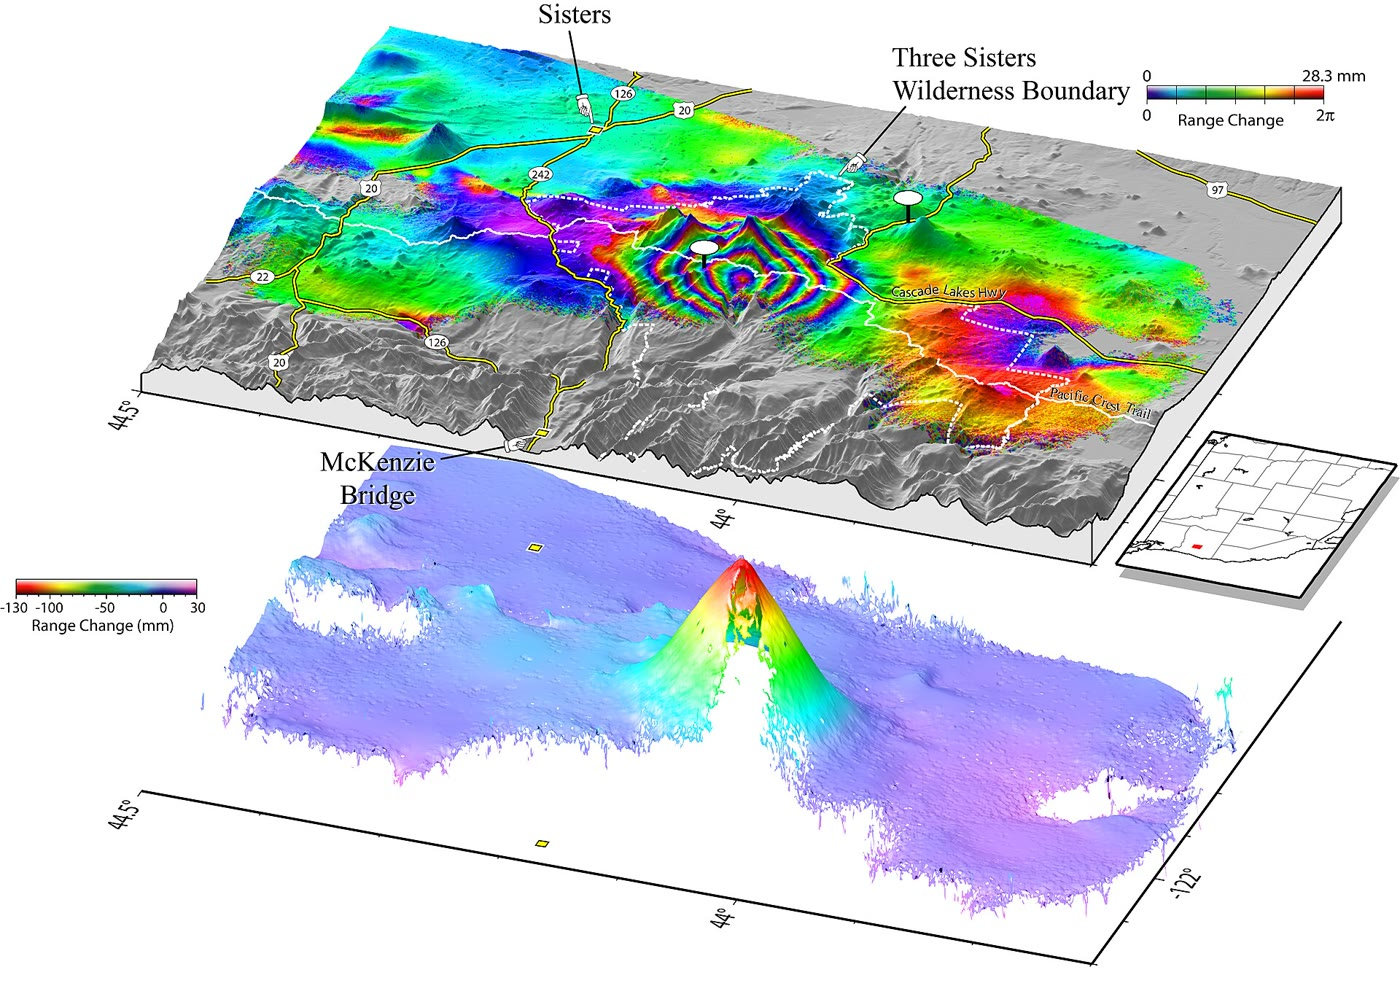
\includegraphics[width=0.86\linewidth]{images/book5/b3-three-sisters-insar.jpg}
\par\smallskip{\small 上图为俄勒冈州三姊妹
火山中心 1995--2001 年的\omterm{def:b3:remote-sensing-gis:insar}{干涉图}，叠置于地形起伏之上：每个颜色循环
代表 \qty{28.3}{mm} 的距离变化，中心处的环状
条纹标示隆起。下图为同一数据经解缠后绘成的
地形图：中心处距离缩短最多达 \qty{130}{mm}。美国
地质调查局（Wicks 等，2002），公有
领域。}\label{fig:b3:remote-sensing-gis:three-sisters}
\end{omfigure}
% ledger: photo:b3-three-sisters-insar, usgs:insar-fs

\begin{inthelab}[地面站]
\begin{minipage}[t]{0.55\linewidth}\vspace{0pt}
成像卫星所记录的数据远多于其在经过成像区域时能发回的量。
Sentinel-1 卫星的雷达每轨道最多可成像半小时，
并将数据存储在星上，存储容量最多达 1410 吉比特；
以两个通道下传，每个通道每秒 260 兆比特，
因此存满的数据约需 45 分钟才能下传完毕。地面站负责接收数据：
卫星升出地平线时，天线
转向对准卫星，跟随其横穿天空，卫星落下时便停止跟踪，
操作人员同时核对数据流是否完整收到。随后
数据被送往处理中心，原始回波在那里变为图像。
\end{minipage}\hfill
\begin{minipage}[t]{0.42\linewidth}\vspace{0pt}
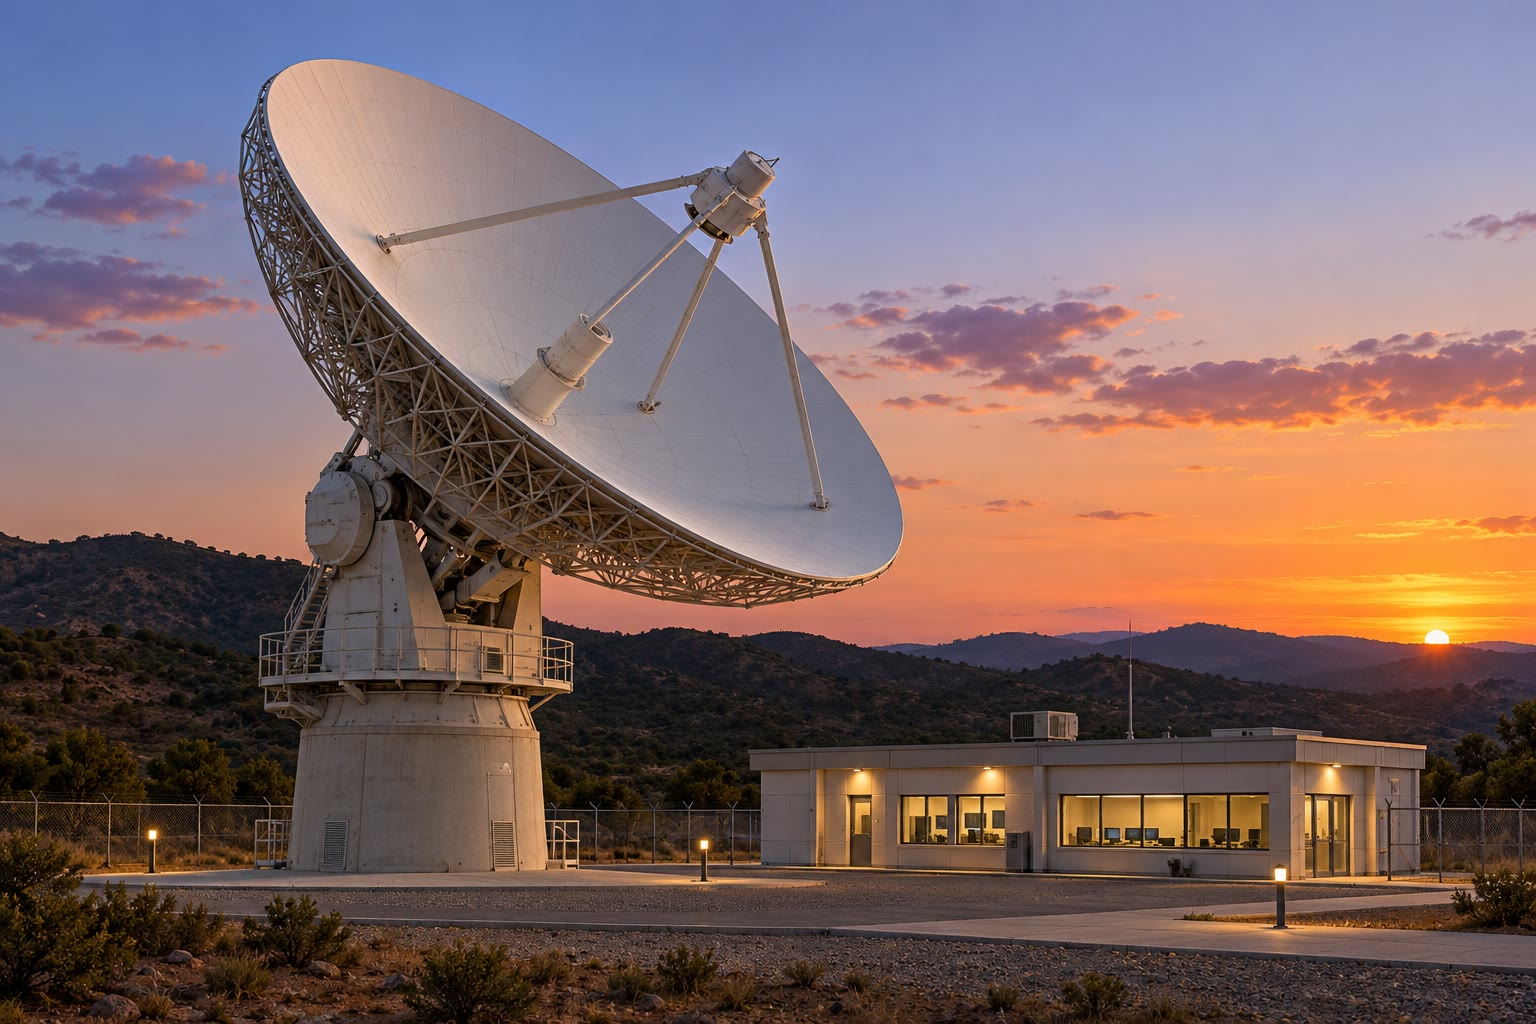
\includegraphics[width=\linewidth]{images/book5/ai/b3-ground-station.jpg}

{\scriptsize 黄昏时的卫星地面站：一座大型跟踪天线及
其运行楼（AI 生成示意图）。}
\end{minipage}
\end{inthelab}
% ledger: esa:s1-downlink

\section{地理信息系统}\label{sec:b3:remote-sensing-gis:gis}

卫星图像、地面的高程模型、
地质图、水井和道路，都是同一地理信息系统的图层，
该系统将它们存储于同一坐标框架中，
并对其进行计算。

\begin{definition}[栅格数据与矢量数据]\label{def:b3:remote-sensing-gis:data-models}
\emph{栅格数据}\index{栅格数据}以单元格构成的网格表示一个图层，
每个单元格存放一个值：反射率、高程或类别。
\emph{矢量数据}\index{矢量数据 (GIS)}则用点、线和多边形表示，
它们由顶点的坐标给出，每个对象
在表中带有一行属性。
\end{definition}

\begin{omfigure}
\centering
\begin{tikzpicture}[x=0.5cm, y=0.5cm, font=\scriptsize]
\begin{scope}
\draw[black!40] (0,0) rectangle (10,7);
\fill[omSea!50, draw=omDef, thick] (3,4.5) ellipse (1.8 and 1.2);
\draw[omDef, very thick] (4.8,4.5) -- (7,3.5) -- (10,2);
\fill[red!70!black] (7,5.5) circle (0.14); \fill[red!70!black] (2,1.5) circle (0.14);
\node[anchor=south] at (5,7.1) {矢量};
\node at (3,4.5) {湖泊};
\node[anchor=south west] at (7.1,5.6) {水井 1};
\node[anchor=south west] at (2.1,1.6) {水井 2};
\node[anchor=north east] at (9.9,2.2) {河流};
\end{scope}
\begin{scope}[xshift=6.5cm]
\foreach \i/\j in {1/4,2/4,3/4,4/4,2/3,3/3,2/5,3/5} {\fill[omSea!50] (\i,\j) rectangle ++(1,1);}
\foreach \i/\j in {5/4,6/3,7/3,8/2,9/2} {\fill[omDef!70] (\i,\j) rectangle ++(1,1);}
\foreach \i/\j in {7/5,2/1} {\fill[red!70!black] (\i,\j) rectangle ++(1,1);}
\draw[black!30, step=1] (0,0) grid (10,7);
\draw[black!40] (0,0) rectangle (10,7);
\node[anchor=south] at (5,7.1) {栅格};
\end{scope}
\end{tikzpicture}
\par\smallskip{\small 同一幅地图的矢量表示（左：一个多边形、一条线和两个点，位置精确，各带其属性）
与栅格表示（右：每个单元格一个值，
湖泊由中心位于其内的单元格表示，
河流与水井由其穿过的单元格表示。栅格便于逐格计算；
\omterm{def:b3:remote-sensing-gis:data-models}{矢量图层}保持形状与拓扑关系，
适用于任意比例尺。}\label{fig:b3:remote-sensing-gis:raster-vector}
\end{omfigure}

\begin{definition}[地理配准]\label{def:b3:remote-sensing-gis:georef}
\emph{地理配准}\index{地理配准}是指为图像的每个像元或图形的每个顶点，
在指定投影中赋予地图坐标，
通常借助地面控制点拟合一个变换，
这些控制点在两种坐标系中的位置均已知。
\end{definition}

在投影坐标框架中，对于北向朝上的栅格，变换为仿射变换：
第 $i$ 列第 $j$ 行的单元格，其角点位于 $E = E_0 + i\,\Delta$，
$N = N_0 - j\,\Delta$，其中 $\Delta$ 为单元格大小。卫星图像需先
重采样为此类网格；不同投影的图层
在合并前须投影到同一投影下。

\begin{method}[由数字高程模型求坡度、坡向与山体阴影]\label{met:b3:remote-sensing-gis:slope}
在高程网格 $z_{i,j}$ 上（间距为 $\Delta$，$i$ 向东，$j$
向北），用中心差分估计梯度，
\[
\frac{\partial z}{\partial x} \approx \frac{z_{i+1,j} - z_{i-1,j}}{2\Delta} ,
\qquad
\frac{\partial z}{\partial y} \approx \frac{z_{i,j+1} - z_{i,j-1}}{2\Delta} .
\]
\emph{坡度}为 $S = \arctan|\nabla z|$；\emph{坡向}是
最陡下降方向的方位角，即 $-\nabla z$ 的方向，$A =
\operatorname{atan2}(-\partial z/\partial x, -\partial z/\partial y)$
从北向顺时针量取。\emph{山体阴影}是指来自方位角
$A_0$、天顶角为 $Z$ 的光源时的值，为 $\cos Z\cos S + \sin Z\sin S
\cos(A_0 - A)$，即光线与地面法线夹角的余弦，
在为负的地方取为零。
\end{method}

中心差分对平面精确，否则误差为
$\Delta^2 z'''/6$；瓦尔登丘陵的晕渲地形图
本科一年级分册中用此法计算，光源位于西北。导数
会放大网格的误差：行与行之间有台阶的模型，
其坡度图上会以条纹形式显示。

\begin{definition}[地图代数]\label{def:b3:remote-sensing-gis:map-algebra}
\emph{地图代数}\index{地图代数}是指计算新的\omterm{def:b3:remote-sensing-gis:data-models}{栅格图层}，
逐单元格由同一网格上的一个或多个图层算得，方法包括算术运算
（由两个波段算出的 NDVI）、比较（坡度大于
\ang{15} 的单元格）、逻辑运算（与、或、非），或
由单元格邻域计算（如坡度）。
\end{definition}

\begin{definition}[缓冲区；叠加分析]\label{def:b3:remote-sensing-gis:operations}
要素在距离 $d$ 处的\emph{缓冲区}\index{缓冲区 (GIS)}是
地图上距其 $d$ 以内的区域。
\emph{叠加分析}\index{叠加分析 (GIS)}将同一区域的两个或多个图层合并为一层，
结果中每个位置带有所有这些图层的属性；
其中最常用的是筛选出
同时满足多个条件的位置。
\end{definition}

\begin{omfigure}
\centering
\begin{tikzpicture}
\begin{groupplot}[group style={group size=2 by 2, horizontal sep=2.0cm, vertical sep=1.5cm},
  width=0.43\linewidth, axis equal image, enlargelimits=false,
  xmin=0, xmax=10, ymin=0, ymax=8,
  tick label style={font=\scriptsize}, label style={font=\small}, title style={font=\small}]
\nextgroupplot[title={(a) 坡度（度）}, ylabel={北向 (km)}, colormap/viridis,
  point meta min=0, point meta max=24, colorbar right,
  colorbar style={width=0.18cm, ytick={0,5,10,15,20}, tick label style={font=\tiny}, axis equal=false}]
\addplot[matrix plot*, mesh/cols=101, point meta=explicit] table[x=x, y=y, meta=slope] {figdata/out/bachelor-3-varden_gis-grid.dat};
\addplot[white, thick] table {figdata/out/shared-region-river.dat};
\nextgroupplot[title={(b) 坡向},
  colormap={aspect}{rgb255=(220,20,30) rgb255=(240,200,0) rgb255=(30,170,60) rgb255=(30,90,220) rgb255=(220,20,30)},
  point meta min=0, point meta max=360, colorbar right,
  colorbar style={width=0.18cm, ytick={0,90,180,270,360}, yticklabels={北, 东, 南, 西, 北}, tick label style={font=\tiny}, axis equal=false}]
\addplot[matrix plot*, mesh/cols=101, point meta=explicit] table[x=x, y=y, meta=aspect] {figdata/out/bachelor-3-varden_gis-grid.dat};
\addplot[black, thick] table {figdata/out/shared-region-river.dat};
\nextgroupplot[title={(c) 两个图层}, xlabel={东向 (km)}, ylabel={北向 (km)},
  colormap={lay}{rgb255=(245,245,245) rgb255=(150,150,150) rgb255=(225,195,140) rgb255=(120,70,20)},
  colormap access=piecewise constant, point meta min=-0.5, point meta max=3.5,
  legend columns=2, legend style={font=\tiny, at={(0.5,-0.3)}, anchor=north, /tikz/every even column/.append style={column sep=4pt}}]
\addplot[matrix plot*, mesh/cols=101, point meta=explicit, forget plot] table[x=x, y=y, meta=layers] {figdata/out/bachelor-3-varden_gis-grid.dat};
\addplot[omDef, thick, forget plot] table {figdata/out/shared-region-river.dat};
\addlegendimage{area legend, fill={rgb,255:red,150;green,150;blue,150}, draw=black!40}
\addlegendentry{坡度大于 \ang{15}}
\addlegendimage{area legend, fill={rgb,255:red,225;green,195;blue,140}, draw=black!40}
\addlegendentry{页岩}
\addlegendimage{area legend, fill={rgb,255:red,120;green,70;blue,20}, draw=black!40}
\addlegendentry{两者}
\nextgroupplot[title={(d) 叠加结果}, xlabel={东向 (km)},
  colormap={cls}{rgb255=(245,245,245) rgb255=(225,195,140) rgb255=(190,150,90) rgb255=(200,20,30)},
  colormap access=piecewise constant, point meta min=-0.5, point meta max=3.5,
  legend columns=2, legend style={font=\tiny, at={(0.5,-0.3)}, anchor=north, /tikz/every even column/.append style={column sep=4pt}}]
\addplot[matrix plot*, mesh/cols=101, point meta=explicit, forget plot] table[x=x, y=y, meta=class] {figdata/out/bachelor-3-varden_gis-grid.dat};
\addplot[omDef, thick, forget plot] table {figdata/out/shared-region-river.dat};
\addplot[black, thin, dashed, unbounded coords=jump] table[x=x, y=y] {figdata/out/bachelor-3-varden_gis-buffer.dat};
\addlegendentry{\qty{1}{km} 缓冲区}
\addlegendimage{area legend, fill={rgb,255:red,225;green,195;blue,140}, draw=black!40}
\addlegendentry{页岩}
\addlegendimage{area legend, fill={rgb,255:red,190;green,150;blue,90}, draw=black!40}
\addlegendentry{缓冲区内的页岩}
\addlegendimage{area legend, fill={rgb,255:red,200;green,20;blue,30}, draw=black!40}
\addlegendentry{选中区域}
\end{groupplot}
\end{tikzpicture}
\par\smallskip{\small 瓦尔登丘陵的一次地理信息系统分析，基于其高程模型，
网格间距 \qty{100}{m}。(a)~坡度，最大达 \ang{23}，出现在谷
坡上；(b)~坡向，即地面所朝方向，河流两岸
彼此相对；(c)~两个图层，坡度大于 \ang{15} 的单元格
与侏罗纪页岩的露头；(d)~二者与河流的
\qty{1}{km} \omterm{def:b3:remote-sensing-gis:operations}{缓冲区}（虚线）叠加：河流上方的陡峭
页岩 \qty{0.32}{km^2}，是可能发生
滑坡的地面的初步筛查。}\label{fig:b3:remote-sensing-gis:varden}
\end{omfigure}

上图完整展示了整个流程：先对高程网格做\omterm{def:b3:remote-sensing-gis:map-algebra}{地图代数}运算，
得到坡度和坡向；再通过比较，把坡度转化为一个图层，
即陡坡单元格；地质图给出页岩；河流的\omterm{def:b3:remote-sensing-gis:operations}{缓冲区}
给出第三个图层；两者的交集，即以逻辑
\emph{与}运算做叠加，在 8181 个单元格中留下 32 个。结果的可靠程度
取决于图层：网格较粗时，坡度偏缓，通过的单元格也更少。

\begin{definition}[监督分类；混淆矩阵]\label{def:b3:remote-sensing-gis:classification}
称\emph{监督分类}\index{监督分类}为
将图像的每个像元归入一组类别之一，依据是
由地面类别已知的训练像元学得的规则或统计量。
其\emph{混淆矩阵}\index{混淆矩阵}对一组独立的参考像元，统计
各真实类别的像元被划入每一类别的数目：
$n_{ij}$ 为被分为 $i$ 类而真实属于 $j$ 类的像元数。
\end{definition}

对角线上为分类正确的像元。设参考像元数为 $N$，
则\emph{总体精度}为 $\sum_i n_{ii}/N$。某类的\emph{用户精度}
为 $n_{ii}$ 与该类行合计之比，即地图判为 $i$ 的像元确为 $i$ 类的概率；
其\emph{生产者精度}为 $n_{ii}$ 与该类列合计之比，
即真实属于 $i$ 类的像元被正确标为 $i$ 类的概率。
\emph{Kappa}系数比较总体精度 $p_o$ 与
随机分配（边缘合计相同）所能达到的精度 $p_e = \sum_i (\text{行}_i)(\text{列}_i)/N^2$，
于是 $\kappa = (p_o - p_e)/(1 -
p_e)$。

\begin{center}
\small
\begin{tabular}{l|ccc|c}
\hline
分类结果 \textbackslash{} 参考 & 水体 & 森林 & 裸岩 & 合计 \\
\hline
水体 & 45 & 2 & 0 & 47 \\
森林 & 3 & 38 & 7 & 48 \\
裸岩 & 0 & 5 & 30 & 35 \\
\hline
合计 & 48 & 45 & 37 & 130 \\
\hline
\end{tabular}
\end{center}

这是一个虚构的例子：130 个像元中有 113 个分类正确，总体精度
为 \qty{86.9}{\percent}。森林的用户精度为
$38/48 = \qty{79}{\percent}$，而生产者精度为 $38/45 =
\qty{84}{\percent}$。有 7 个裸岩像元（或许处于阴影中）被
判为森林。随机分配将达到 $p_e = 0.338$，因而 $\kappa =
0.80$。

\section{练习}

\begin{exercise}[$\star$]\label{exo:b3:remote-sensing-gis:1}
某农田在成像仪的红光波段反射率为 0.06，近红外波段为 0.42；
与其相邻的一块耕地在两波段的反射率分别为 0.21 和 0.28。
分别计算两者的 NDVI，并说明各自的数值表明什么。
\end{exercise}

\begin{exercise}[$\star$]\label{exo:b3:remote-sensing-gis:2}
Landsat~8 成像仪的扫描带宽为 \qty{185}{km}，像元大小为 \qty{30}{m}，
全色波段像元为 \qty{15}{m}。(a)~两种情况下，横跨扫描带的一行各含多少像元？
(b)~12 位和 8 位各能给出多少个量化等级？
(c)~仅由 Landsat~8 工作时的\omterm{def:b3:remote-sensing-gis:resolutions}{重访周期}为多少，
以及 Landsat~8 与 Landsat~9 合用时为多少？
\end{exercise}

\begin{exercise}[$\star$]\label{exo:b3:remote-sensing-gis:3}
(a)~在一幅 Sentinel-1 \omterm{def:b3:remote-sensing-gis:insar}{干涉图}（$\lambda = \qty{5.55}{cm}$）上，
某一沉降盆地中，6 条干涉条纹把稳定边缘与中心隔开。
中心处\omterm{def:b3:remote-sensing-gis:insar}{视线方向}的变化为多少？(b)~若用波长为 \qty{5.66}{cm} 的较老卫星，
一条干涉条纹对应的变化为多少？
\end{exercise}

\begin{exercise}[$\star$]\label{exo:b3:remote-sensing-gis:4}
激光高度计距地面 \qty{500}{km}。(a)~一个脉冲返回所需的时间为多少？
(b)~若每个光子的计时精度为 \qty{800}{ps}，
则一次测距的精确度有多高？
\end{exercise}

\begin{exercise}[$\star\star$]\label{exo:b3:remote-sensing-gis:5}
Landsat~8 第~10~波段（取 $\lambda = \qty{10.9}{\micro\metre}$）的一个像元，
经\omterm{def:b3:remote-sensing-gis:atm-correction}{大气校正}后，其光谱辐亮度为
\qty{9.0}{W.m^{-2}.sr^{-1}.\micro\metre^{-1}}。(a)~计算其\omterm{def:b3:remote-sensing-gis:brightness}{亮
度温度}。(b)~地表为发射率 0.98 的草地，其
动力学温度为多少？
\end{exercise}

\begin{exercise}[$\star\star$]\label{exo:b3:remote-sensing-gis:6}
Sentinel-1 雷达卫星飞行在 \qty{693}{km} 高空，天线长 \qty{12.3}{m}，
工作波长 $\lambda = \qty{5.55}{cm}$。(a)~忽略地球曲率，
计算入射角为
\ang{35} 时所观测一点的斜距。(b)~若用同样长的真实天线，其方位向分辨率为多少，
合成孔径又能给出多少？(c)~合成
孔径的长度为多少？
\end{exercise}

\begin{exercise}[$\star\star$]\label{exo:b3:remote-sensing-gis:7}
数字高程模型中的一个 $3\times3$ 窗口，单元格边长为 \qty{30}{m}，
北方在上，读数如下：
\[
\begin{matrix} 412 & 418 & 425 \\ 405 & 410 & 418 \\ 398 & 401 & 409 \end{matrix}
\qquad (\unit{m}).
\]
用中心差分法计算中心单元格的坡度和坡向，
以及西北方向、高出地平线 \ang{45} 的光源下的
山体阴影。
\end{exercise}

\begin{exercise}[$\star\star$]\label{exo:b3:remote-sensing-gis:8}
用 160 个参考像元检验一幅土地覆盖图（行为地图，
列为真实情况；类别为水体、森林、农田、城镇）：
\[
\begin{pmatrix} 48 & 3 & 1 & 0 \\ 4 & 37 & 6 & 1 \\ 2 & 5 & 29 & 2 \\ 0 & 1 & 2 & 19 \end{pmatrix} .
\]
计算总体精度、各类别的用户精度与生产者精度，
以及 Kappa 系数；哪一类最常被漏判？
\end{exercise}

\begin{exercise}[$\star\star$]\label{exo:b3:remote-sensing-gis:9}
一个 \qty{100}{m} 热红外像元中含有一股新近形成的熔岩流，温度为 \qty{1443}{K}
覆盖其中 \qty{4}{\percent}；其余为温度 \qty{290}{K} 的地面，二者都
视为黑体。(a)~计算该像元在
\qty{10.9}{\micro\metre} 处的\omterm{def:b3:remote-sensing-gis:brightness}{亮度温度}，并与平均温度比较。
(b)~计算熔岩与地面在
\qty{2.2}{\micro\metre} 处的黑体辐射亮度之比，以及该像元在此波长的
\omterm{def:b3:remote-sensing-gis:brightness}{亮度温度}。哪一波段更能探测到熔岩？
\end{exercise}

\begin{exercise}[$\star\star\star$]\label{exo:b3:remote-sensing-gis:10}
同一形变的两幅\omterm{def:b3:remote-sensing-gis:insar}{干涉图}由两次过境获取，一次卫星位于地面以东，
另一次位于西侧，两次入射角均为 \ang{35}。某一点的
\omterm{def:b3:remote-sensing-gis:insar}{视线方向}在第一幅图中缩短 \qty{64}{mm}，在第二幅图中
缩短 \qty{38}{mm}。假设无南北向运动，计算该点的竖直
位移与向东位移。
为什么仅一次过境不够？
\end{exercise}

\begin{exercise}[$\star\star\star$]\label{exo:b3:remote-sensing-gis:11}
\omterm{def:b3:remote-sensing-gis:insar}{相位解缠}在相邻像元之间相位跳变超过 $\pi$ 时失效。
(a)~证明\omterm{def:b3:remote-sensing-gis:insar}{视线方向}在相邻像元之间的变化必须小于 $\lambda/4$，
对 Sentinel-1 为 \qty{13.9}{mm}。
(b)~对位于 $z_0 = \qty{4}{km}$ 处的茂木源，$\Delta V =
\qty{e7}{m^3}$，$\nu = 0.25$，从竖直方向观测，证明
$u_z$ 的最陡梯度出现在 $r = z_0/2$ 处，并计算它。(c)~
保持条纹可分辨的最大像元尺寸是多少？
\end{exercise}

\begin{exercise}[$\star\star\star$]\label{exo:b3:remote-sensing-gis:12}
(a)~证明：对非负反射率，NDVI 位于 $-1$ 与 $+1$ 之间，
并证明当两个反射率都
乘以同一因子时 NDVI 保持不变。(b)~草地的反射率：红波段为 0.051，
近红外为 0.502。未经校正的影像会附加路径辐射，
其值相当于红波段 0.03、近红外 0.01。计算有、无该项时的
NDVI。(c)~这对于由未经校正的雾霾天影像所制的 NDVI 图
意味着什么？
\end{exercise}

\section{问题：哈尔夫伦山上一处肿胀的山侧}

\begin{problem}[{周末问题——植被、热量与雷达
干涉图：一座虚构火山}]
\label{pb:b3:remote-sensing-gis:1}
哈尔夫伦山是一座虚构的火山，曾在 1890、1960
和 2005 年向其森林覆盖的山侧喷出熔岩流。山顶的喷气孔区正冒着蒸汽。
下面给出近期某一年的卫星数据。

\medskip\noindent\textbf{第一部分——熔岩流上的植被。}经校正的
红波段与近红外波段反射率：
\begin{center}
\small
\begin{tabular}{lcccc}
\hline
地表 & 森林 & 1890 年熔岩流 & 1960 年熔岩流 & 2005 年熔岩流 \\
\hline
红波段 & 0.04 & 0.07 & 0.11 & 0.12 \\
近红外 & 0.38 & 0.30 & 0.21 & 0.14 \\
\hline
\end{tabular}
\end{center}
\begin{enumerate}
\item 计算四种地表的 NDVI。
\item 按植被恢复程度对各熔岩流排序。该排序
  是否与其年龄顺序一致？
\item 为什么 2005 年熔岩流的 NDVI 不为零，
  尽管其上几乎没有植物生长？
\item 为什么 NDVI 比单独的近红外反射率
  在陡峭、光照不均的火山侧翼上更可靠？
\end{enumerate}

\medskip\noindent\textbf{第二部分——喷气孔区。}在热红外
波段（取 $\lambda = \qty{10.9}{\micro\metre}$）中，经校正的
远离喷气孔的山顶台地上一个 \qty{100}{m} 像元的辐亮度为
\qty{8.40}{W.m^{-2}.sr^{-1}.\micro\metre^{-1}}，而喷气孔区上方像元的辐亮度为
\qty{9.95}{W.m^{-2}.sr^{-1}.\micro\metre^{-1}}。
\begin{enumerate}[resume]
\item 计算两个像元的\omterm{def:b3:remote-sensing-gis:brightness}{亮度温度}。
\item 台地岩石的发射率为 0.97。其
  动力学温度是多少？
\item 喷气口及其周围的暖地表温度均为
  \qty{370}{K}。将它们及其余部分视为黑体，其余部分取台地的辐亮度，
  它们占像元的比例为多少，
  面积又为多少？
\item 为什么像元按面积加权的平均温度
  低于其\omterm{def:b3:remote-sensing-gis:brightness}{亮度温度}？
\end{enumerate}

\medskip\noindent\textbf{第三部分——\omterm{def:b3:remote-sensing-gis:insar}{干涉图}。}两幅 Sentinel-1
影像（$\lambda = \qty{5.55}{cm}$，入射角 \ang{35}，卫星位于
东侧）相隔 48 天拍摄，显示东侧山侧上有一个靶心状图案。从一个
稳定区域到图案中心，共数得五条完整条纹和
第六条条纹的十分之四，它们均表示朝向
卫星的运动。
\begin{enumerate}[resume]
\item 为什么两幅影像必须从几乎相同的位置获取，
  两者之间相隔同一卫星的多少个轨道循环？
\item 计算中心处\omterm{def:b3:remote-sensing-gis:insar}{视线方向}的变化量。
\item 中心处地面只发生竖直运动，计算该处的
  隆升量。
\item 解释图案为何不是圆形，并说明条纹在哪一侧
  更密集，是东侧还是西侧？
\item 沿穿过中心的南北向直线，\omterm{def:b3:remote-sensing-gis:insar}{视线方向}的变化
  降为中心值一半的点距中心 \qty{3.4}{km}。
  为何采用该直线？它给出的茂木源
  深度是多少？
\item 中心与该半高点之间相隔多少条条纹？
\item 大气中的水蒸气可使雷达波在两个日期上的延迟
  不同，并形成其自身的条纹。另一对日期的第二幅\omterm{def:b3:remote-sensing-gis:insar}{干涉图}
  如何有助于区分两者？
\end{enumerate}

\medskip\noindent\textbf{第四部分——体积变化。}取 $\nu = 0.25$。
\begin{enumerate}[resume]
\item 由 $u_z(0) = (1 - \nu)\Delta V/(\pi z_0^2)$，计算源的
  体积变化量。
\item 将其表示为 48 天内的平均每日速率及每年速率。
\item 计算最大水平位移及其出现的位置。
\item 若储库为半径 $z_0/3$ 的球体，其体积
  将是多少？该变化量占其中的多大比例？
\item 半径为 $z_0/3$ 的球体的有限尺寸使隆升量
  改变约 \qty{3}{\percent}。考虑到条纹计数的精度，第~16~问的答案
  是否有明显变化？
\item 除第一、二部分的数据或地面观测外，还有
  什么观测可支持储库正在充填的解释？
\item 给出哈尔夫伦山下储库的体积变化，
  以百万立方米为单位，保留两位有效数字。
\end{enumerate}
\end{problem}
% ledger: nasa:ndvi, esa:s1-sar, esa:s1-orbit, esa:s1-iw, dmodels:mogi, dmodels:mogi-radial, const:h, const:c, const:kB
